% Created 2024-04-28 Κυρ 19:37
% Intended LaTeX compiler: pdflatex
\documentclass[11pt]{article}
\usepackage[utf8]{inputenc}
\usepackage[T1]{fontenc}
\usepackage{graphicx}
\usepackage{longtable}
\usepackage{wrapfig}
\usepackage{rotating}
\usepackage[normalem]{ulem}
\usepackage{amsmath}
\usepackage{amssymb}
\usepackage{capt-of}
\usepackage{hyperref}
\usepackage{booktabs}
\usepackage{import}
\usepackage[LGR, T1]{fontenc}
\usepackage[greek, english, american]{babel}
\usepackage{alphabeta}
\usepackage{esint}
\usepackage{mathtools}
\usepackage{esdiff}
\usepackage{makeidx}
\usepackage{glossaries}
\usepackage{newfloat}
\usepackage{minted}
\usepackage[a4paper, margin=3cm]{geometry}
\usepackage{chemfig}
\usepackage{svg}
\author{Vidianos Giannitsis}
\date{\today}
\title{Εισαγωγή - Στατιστικά Στοιχεία}
\hypersetup{
 pdfauthor={Vidianos Giannitsis},
 pdftitle={Εισαγωγή - Στατιστικά Στοιχεία},
 pdfkeywords={},
 pdfsubject={},
 pdfcreator={Emacs 29.3 (Org mode 9.6.15)}, 
 pdflang={English}}
\makeatletter
\newcommand{\citeprocitem}[2]{\hyper@linkstart{cite}{citeproc_bib_item_#1}#2\hyper@linkend}
\makeatother

\usepackage[notquote]{hanging}
\begin{document}

\maketitle
\tableofcontents


\section{List}
\label{sec:orgf164e19}
\listoffigures

\section{Εισαγωγή}
\label{sec:org15c371b}
Τα υπολείμματα τροφών αποτελούν μία από τις σημαντικότερες κατηγορίες οργανικών αποβλήτων. Ο οργανισμός τροφίμων και αγρονομίας των ηνωμένων πολιτείων (FAO) υπολογίζει πως περίπου το 1/3 της παγκόσμιας παραγωγής τροφών (περίπου 1.3 δις τόνοι ετησίως) χάνεται κατά την παραγωγική διαδικασία ή απορρίπτεται (Ishangulyyev, Kim, and Lee 2019).

Συγκεκριμένα, έχει προσδιοριστεί πως το ισοδύναμο διοξειδίου του άνθρακα που παράγεται λόγω της μη ορθής αυτής διαχείρισης των υπολείμματων ανέρχεται στους 3.3 δις τόνους (Taheri et al. 2021) . Ακόμη, έχει βρεθεί πως τα υπολείμματα τροφών που οφείλονται μόνο στην απόρριψη τροφών από καταναλωτές σε ανεπτυγμένες χώρες είναι σχεδόν όσα παράγουν οι υπό σακχάριες και αφρικανικές χώρες συνολικά (περίπου 230 εκατομμύρια). Οπότε η αποφυγή της δημιουργίας τόσων υπολειμμάτων - ή η καλύτερη αξιοποίηση τους - θα μπορούσε να λύσει πολλά προβλήματα υποσιτισμού. Ακόμη και στον οικονομικό τομέα, δημιουργούνται σοβαρά προβλήματα από την ανεξέλεγκτη αυτή απόρριψη καθώς η καθαρή αξία των τροφών που χάνονται ή απορρίπτονται σε κάποιο σημείο της εφοδιαστικής αλυσίδας είναι 936 δις δολλάρια ανά έτος με ελάχιστο κέρδος, καθώς πολύ μικρές ποσότητες των υπολειμμάτων αυτών αξιοποιούνται (Ishangulyyev, Kim, and Lee 2019) . Συμπερασματικά, η δημιουργία αυτών των υπέρογκων ποσοτήτων υπολειμμάτων τροφών πλήγει κάθε πυλώνα της βιωσιμότητας και είναι ένα πάρα πολύ σοβαρό πρόβλημα.

Μία από τις βασικότερες υποκατηγορίες υπολειμμάτων τροφών είναι τα οικιακά υπολείμματα τροφών. Αποτελούν το μεγαλύτερο κομμάτι της παγκόσμιας παραγωγής υπολειμμάτων τροφών, αποτελώντας περίπου το \(61 \%\) αυτής (“Statista - The Statistics Portal” n.d.) . Στο \figurename \ref{fig:org5347d6d} φαίνεται η παγκόσμια παραγωγή υπολειμμάτων τροφών ανά τομέα.
\begin{figure}[htbp]
\centering
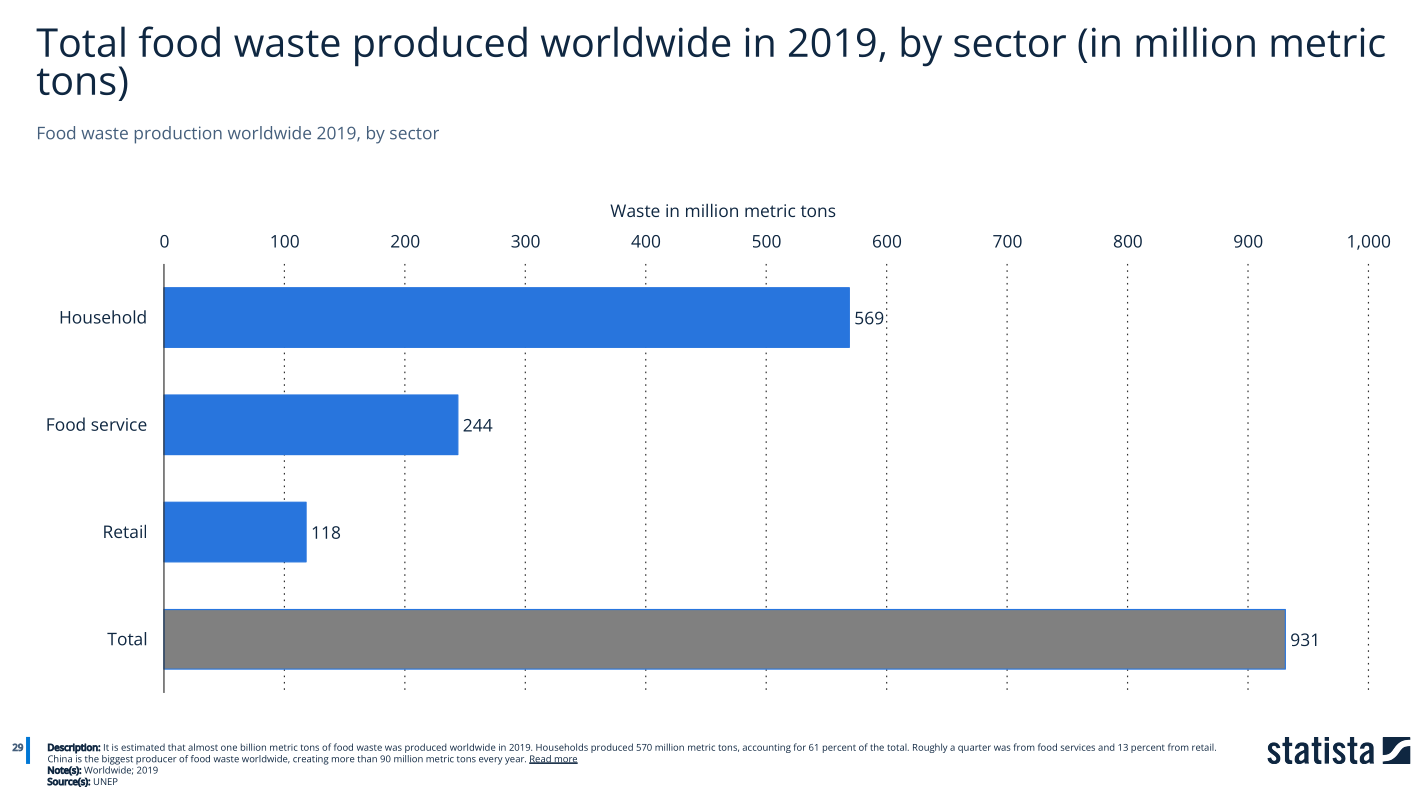
\includegraphics[width=.9\linewidth]{../plots/statistics/statistic_food_waste_by_sector_2019.png}
\caption{\label{fig:org5347d6d}Παγκόσμια παραγωγή υπολειμμάτων τροφών ανά τομέα}
\end{figure}

Η Ελλάδα είναι η χώρα με την δεύτερη μεγαλύτερη παραγωγή οικιακών υπολειμμάτων τροφών κατά κεφαλήν παγκοσμίως (142 κιλά/άτομο ετησίως) (“Statista - The Statistics Portal” n.d.) . Η παραγωγή υπολειμμάτων τροφών, ειδικά στον τομέα της κατανάλωσης, όπου βρίσκονται τα οικιακά υπολείμματα, καθώς και αυτά της εστίασης, είναι πολύ συχνά αναπόφευχτη. Οπότε, παρόλο που με πιο σωστές πρακτικές θα μπορούσαν να παράγονται λιγότερα υπολείμματα, η ανάπτυξη τεχνολογιών αξιοποίησης των υπολειμμάτων αυτών είναι πάρα πολύ σημαντικές. Οι τεχνολογίες αυτές θα πρέπει να είναι εύκολα εφαρμόσιμες και οικονομικές και η κλιμάκωση τους να είναι εφικτή.

Η αγορά της διαχείρισης αποβλήτων είναι αρκετά μεγάλη (υπολογίζεται περίπου στα 1293 δις δολλάρια ετησίως από μία μελέτη του 2022), ενώ προβλέψεις λένε πως θα φτάσει τα 2000 δις μέχρι το 2030. Κομμάτι της ανάπτυξης αυτής, θα πρέπει να είναι και η ανάπτυξη βιώσιμων τεχνολογιών αξιοποίησης απορριμμάτων, καθώς αυτή την στιγμή, με εξαίρεση τα απορρίμματα τα οποία είναι ανακυκλώσιμα, οι βασικές τεχνολογίες που εφαρμόζονται είναι η ανάκτηση ενέργειας μέσω καύσης και η διάθεση των απορριμμάτων σε χώρους υγειονομικής ταφής (ΧΥΤΑ) όπως φαίνεται και στο \figurename  \ref{fig:org22664b2} (“Statista - The Statistics Portal” n.d.).

\begin{figure}[htbp]
\centering
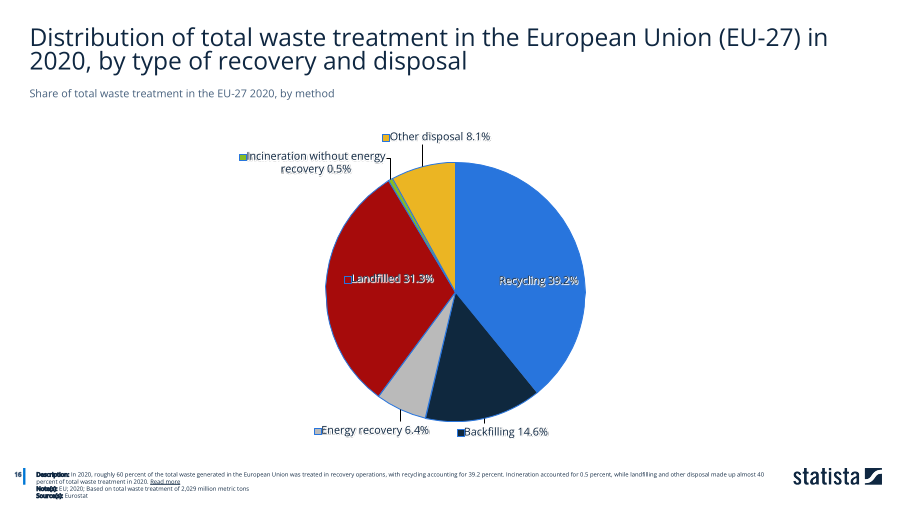
\includegraphics[width=.9\linewidth]{../plots/statistics/statistic_waste_treatment_technologies_europe_2020.png}
\caption{\label{fig:org22664b2}Τεχνολογίες επεξεργασίας απορριμμάτων στην Ευρωπαική Ένωση}
\end{figure}

Οι τεχνολογίες αυτές χρησιμοποιούνται επειδή είναι πολύ απλές και έχουν χαμηλό κόστος. Στα πλαίσια όμως της βιώσιμης ανάπτυξης και της κυκλικής οικονομίας, πρέπει τα απορρίμματα να εξετάζονται ως μία νέα πρώτη ύλη, από την οποία μπορούν να διυλιστούν προϊόντα αυξημένης αξίας.

Αυτές οι τεχνολογίες μπορεί να είναι θερμικές, όπως η πυρόλυση (Pardo et al. 2023; Usmani et al. 2021) η οποία παράγει ένα προιόν γνωστό ως biochar, το οποίο έχει πολύ χρήσιμες ιδιότητες (Xu et al. 2024; Infurna, Caruso, and Dintcheva 2023), ή η αεριοποίηση (Usmani et al. 2021; Murugesan et al. 2022), η οποία παράγει ένα μίγμα υδρογόνου και μονοξειδίου του άνθρακα γνωστό ως αέριο σύνθεσης (syngas), το οποίο μπορεί να χρησιμοποιηθεί ως πρώτη ύλη για πολλά προιόντα. Στο \figurename  \ref{fig:org0e9372b} φαίνονται κάποια κλασσικά παραδείγματα αυτού (Udaeta et al. 2007)

\begin{figure}[htbp]
\centering
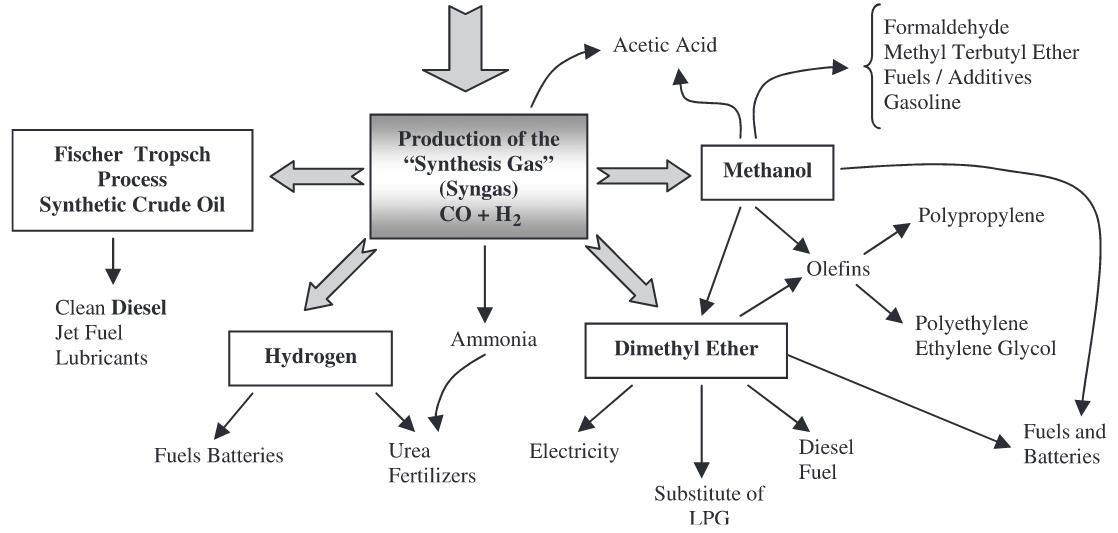
\includegraphics[width=.9\linewidth]{./gasification_products.png}
\caption[Προιόντα του αερίου σύνθεσης]{\label{fig:org0e9372b}Προιόντα του αερίου σύνθεσης (Udaeta et al. 2007)}
\end{figure}

Εκτός από θερμικές τεχνολογίες, υπάρχει μεγάλο ενδιαφέρον στις βιολογικές τεχνολογίες. Αυτές μπορεί να είναι αερόβιες, όπως η κομποστοποίηση, η οποία παράγει ένα εδαφοβελτιωτικό προιόν (Cerda et al. 2018), ή αναερόβιες όπως η αναερόβια χώνευση, η οποία έχει ως κύριο προιόν το βιοαέριο, ένα μίγμα μεθανίου και διοξειδίου του άνθρακα που μπορεί να χρησιμοποιηθεί ως βιοκαύσιμο (Ma et al. 2018; Xu et al. 2018), ή διάφορες διεργασίες ζύμωσης. Σε αυτές υπάγονται η αλκοολική ζύμωση, μία από τις πιό ευρέως χρησιμοποιούμενες τεχνολογίες αξιοποίησης απορριμμάτων (Anwar Saeed et al. 2018; Roukas and Kotzekidou 2022), η σκοτεινή ζύμωση για την παραγωγή υδρογόνου (Yasin et al. 2013; Mohanakrishna et al. 2023), ή οι ζυμώσεις με σκοπό την παραγωγή μονομερών για βιοπολυμερή όπως το πολυγαλακτικό οξύ (PLA) (Rajesh Banu and Godvin Sharmila 2023; Pleissner et al. 2017) .

Η παρούσα μελέτη θα εστιάσει στην αναερόβια χώνευση, καθώς είναι μία τεχνολογία με μεγάλο δείκτη ετοιμότητας (technology readiness level or TRL) (Mankins, n.d.), η οποία έχει εφαρμοστεί επιτυχώς σε μεγάλη κλίμακα και είναι οικονομική. Η αναερόβια χώνευση είναι μία αναερόβια βιολογική διεργασία η οποία διακρίνεται σε 4 στάδια. Στο πρώτο στάδιο, το αρχικό υπόστρωμα της διεργασίας, το οποίο συχνά αποτελείται από περίπλοκα πολυμερή όπως οι υδατάνθρακες, οι πρωτείνες και τα λιπίδια, υδρολύονται σε απλούστερες ενώσεις. Αυτές μπορούν να χρησιμοποιηθούν από τα οξεογόνα βακτήρια τα οποία τα μετατρέπουν σε πτητικά λιπαρά οξέα (VFAs) όπως το οξικό οξύ, το προπιονικό οξύ, το βουτηρικό οξύ ή το γαλακτικό οξύ και σε αλκοόλες όπως η αιθανόλη. Στο 3ο στάδιο, οι ενώσεις αυτές μετατρέπονται σε οξικό οξύ, υδρογόνο και διοξείδιο του άνθρακα κατά την διεργασία της οξεογένεσης, ενώ τελικά, το οξικό οξύ μετατρέπεται σε μεθάνιο από μία κατηγορία μεθανογόνων μικροοργανισμών ενώ το υδρογόνο και το διοξείδιο του άνθρακα μετατρέπονται σε μεθάνιο από μία άλλη κατηγορία μεθανογόνων. Τα στάδια αυτά φαίνονται και στο \figurename \ref{fig:org39a9f7a} (Grippi, Clemente, and Bernal 2020) .

\begin{figure}[htbp]
\centering
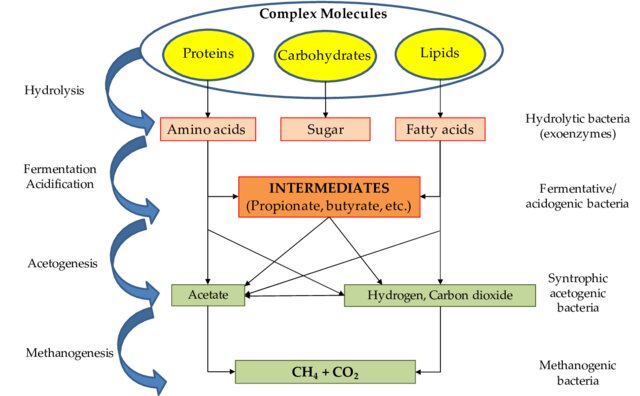
\includegraphics[width=.9\linewidth]{./anaerobic_digestion_phases.jpg}
\caption[Φάσεις της αναερόβιας χώνευσης]{\label{fig:org39a9f7a}Φάσεις της αναερόβιας χώνευσης (Grippi, Clemente, and Bernal 2020)}
\end{figure}

Τα υπολείμματα τροφών είναι ένα πολύ καλό υπόστρωμα για αναερόβια χώνευση καθώς είναι πλούσια σε εύκολα αποδομήσιμες οργανικές ενώσεις αλλά και θρεπτικά στοιχεία και μπορούν να μετατραπούν πολύ αποτελεσματικά σε βιοαέριο. Στο \figurename \ref{fig:org6740cd1} φαίνεται η παγκόσμια παραγωγή ενέργειας από βιοαέριο τα τελευταία 15 χρόνια, η οποία έχει ραγδαία αύξηση (“Statista - The Statistics Portal” n.d.) .

\begin{figure}[htbp]
\centering
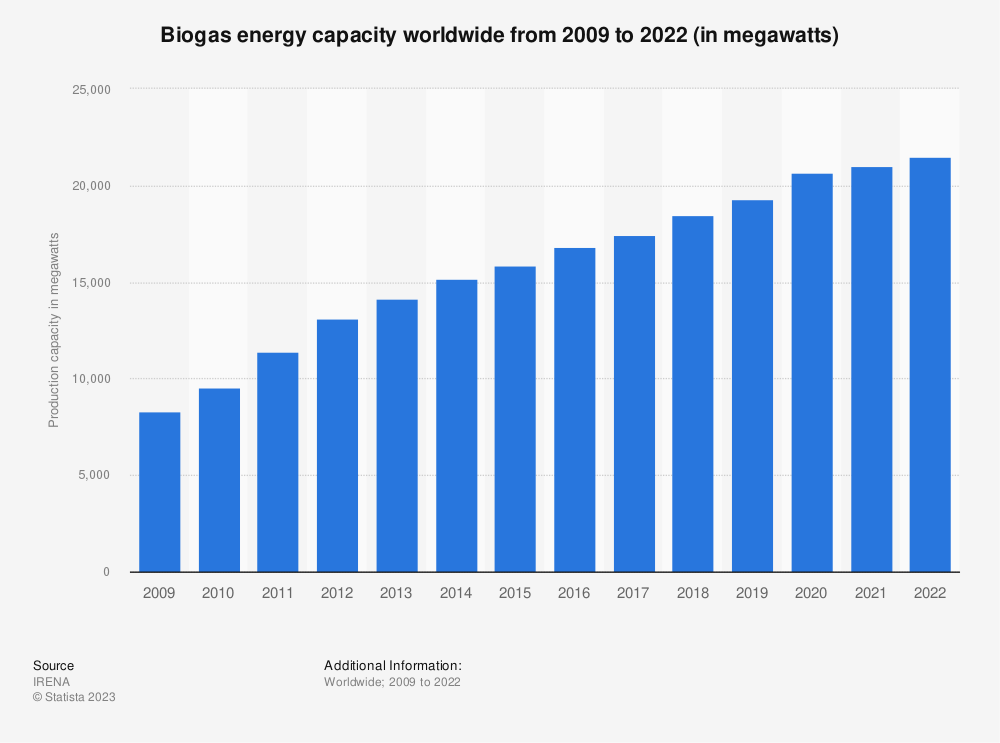
\includegraphics[width=.9\linewidth]{../plots/statistics/statistic_id1032922_global-biogas-energy-capacity-2009-2022.png}
\caption{\label{fig:org6740cd1}Παγκόσμια παραγωγή ενέργειας από βιοαέριο}
\end{figure}

Εκτός όμως από την αξιοποίηση του μεγάλου βιοχημικού δυναμικού των υπολειμμάτων αυτών, η αναερόβια χώνευση λύνει και άλλο ένα από τα σημαντικά προβλήματα του 21ου αιώνα, το οποίο είναι η ενέργεια. Αυτή τη στιγμή, πάνω από το \(80 \%\) της ενέργειας που καταναλώνεται παγκοσμίως βασίζεται σε μη ανανεώσιμες πηγές όπως το πετρέλαιο και το φυσικό αέριο. Οι ενεργειακές απαιτήσεις παγκοσμίως έχουν μία συνεχή αύξηση, ενώ οι πρώτες ύλες αυτές εξαλείφονται (“Statista - The Statistics Portal” n.d.) . Οπότε, τεχνολογίες παραγωγής ενέργειας από ανανεώσιμες πηγές, οι οποίες να έχουν το δυναμικό να αντικαταστήσουν τις πηγές αυτές θα γίνουν απαραίτητες τα επόμενα χρόνια. Οι περισσότερες τεχνολογίες ανανεώσιμης ενέργειας (πχ αιολική, ηλιακή ή υδροηλεκτρική ενέργεια) έχουν δυσκολία να φτάσουν τέτοια επίπεδα και για αυτό χρησιμοποιούνται επικουρικά σε μία κύρια πηγή ενέργειας (αυτή τη στιγμή, περίπου το \(30 \%\) της παγκόσμιας παραγωγής ηλεκτρισμού οφείλεται σε τέτοιες πηγές) (“Statista - The Statistics Portal” n.d.) . Τα υπολείμματα τροφών από την άλλη είναι άφθονα οπότε θεωρείται πως με μία αποτελεσματική επεξεργασία θα μπορέσουν να καλύψουν ένα πολύ σημαντικό ποσοστό της παγκόσμιας ανάγκης σε ενέργεια.

Βέβαια, η αναερόβια χώνευση έχει κάποια σημαντικά λειτουργικά προβλήματα. Ο βασικός περιορισμός της, ο οποίος λειτουργεί πολλά από αυτά τα προβλήματα είναι η ευαισθησία των μεθανογόνων μικροοργανισμών στις περιβαλλοντικές συνθήκες. Λόγω της ευαισθησίας τους, η αναερόβια χώνευση λειτουργεί στις βέλτιστες συνθήκες αυτών. Αυτό όμως οδηγεί στην λιγότερο αποτελεσματική διεξαγωγή των άλλων σταδίων. Το κυριότερο πρόβλημα που δημιουργείται είναι πως η υδρόλυση μπορεί μεν να διεξαχθεί, αλλά γίνεται σε πολύ αργό ρυθμό, καθιστώντας την το περιοριστικό στάδιο της αναερόβιας χώνευσης και τον λόγο για τον οποίο θεωρείται μία αρκετά αργή διεργασία. Ένα αντίστοιχο πρόβλημα υπάρχει και στο στάδιο της οξεογένεσης, όπου οι μικροοργανισμοί δεν λειτουργούν στις βέλτιστες συνθήκες τους και μπορούν να ακολουθήσουν μόνο ένα μεταβολικό μονοπάτι, το οποίο ενεργοποιείται στις συνθήκες που λειτουργούν. Παρόλα αυτά, σε ορισμένες περιπτώσεις, ο ρυθμός της οξεογένεσης ξεπερνάει αυτόν της μεθανογένεσης (ο οποίος είναι γενικά αργός), με αποτέλεσμα να παράγονται υπερβολικές ποσότητες από VFAs, το οποίο οδηγεί σε οξίνιση του αντιδραστήρα και κατάρρευση της διεργασίας καθώς οι μεθανογόνοι δεν μπορούν να λειτουργήσουν σε εκείνες τις τιμές pH (Usmani et al. 2021; Azbar, Ursillo, and Speece 2001; Zoetemeyer et al. 1982).

Ένας τρόπος να επιλυθεί το πρόβλημα αυτό είναι ο διαχωρισμός των σταδίων της υδρόλυσης και της ζύμωσης, σε μία διεργασία δύο (Pohland and Ghosh 1971) ή τριών (Zhang et al. 2017) σταδίων. Αυτό που πετυχαίνεται με τον διαχωρισμό αυτόν είναι να λειτουργούν όλα τα στάδια της διεργασίας στο βέλτιστο σημείο λειτουργίας τους και άρα να είναι πολύ πιο αποτελεσματικά. Επιπροσθέτως, ο αντιδραστήρας δεν οξινίζεται κατά την διάρκεια της μεθανογένεσης, με αποτέλεσμα η διεργασία να είναι πολύ πιο σταθερή. Όμως, υπάρχει το πρόβλημα πως οι διεργασίες αυτές έχουν υψηλότερο κόστος, λόγω του περισσότερου εξοπλισμού, αλλά και πολυπλοκότητας της διεργασίας. Για τον λόγο αυτόν, η διεργασία αναερόβιας χώνευσης πολλαπλών σταδίων έχει πολύ χαμηλότερο TRL και δεν έχει εφαρμοστεί ευρέως σε μεγάλη κλίμακα (Azbar, Ursillo, and Speece 2001; Wu et al. 2022; Ma et al. 2018; Usmani et al. 2021) . 

Ο σκοπός της παρούσας μελέτης είναι να κάνει μία βιβλιογραφική ανασκόπηση των τεχνολογιών αναερόβιας χώνευσης σε πολλαπλά στάδια και με βάση αυτήν να αναπτύξει μία διεργασία αξιοποίησης υπολειμμάτων τροφών η οποία να είναι οικονομικά βιώσιμη αλλά ταυτόχρονα αποτελεσματική. Τα πειράματα που διεξάχθηκαν για τον σκοπό αυτόν έγιναν σε εργαστηριακή κλίμακα όπου υπάρχει πολύ καλός έλεγχος της διεργασίας, αλλά επικυρώθηκαν και σε πιλοτική κλίμακα για να αναδειχθεί η δυνατότητα κλιμάκωσης της προτεινόμενης διεργασίας.
\end{document}
